\documentclass[12pt]{article}

\usepackage[utf8]{inputenc}
\usepackage[left=2cm,right=2cm,top=2cm,bottom=4cm]{geometry}
\usepackage[ngerman]{babel}
\usepackage{amsmath, amsfonts, amssymb, amsthm}
\usepackage{graphicx}
\usepackage{multicol}
\usepackage[compact]{titlesec}
\usepackage{enumitem}
\usepackage{minted}

\usepackage[style=authoryear, backend=biber]{biblatex}
\addbibresource{bibliography.bib}

\usepackage{ulem, contour}
\usepackage{xcolor, colortbl}
\usepackage{caption, subcaption}
\usepackage{listings}
\usepackage{hyperref}
\usepackage[numbib,nottoc]{tocbibind}

\renewcommand{\ULdepth}{1.8pt}
\contourlength{0.8pt}
\newcommand{\cul}[1]{%
  \uline{\phantom{#1}}%
  \llap{\contour{white}{#1}}%
}

\lstset{
    language=tex,
    backgroundcolor=\color{black!5},
    basicstyle=\footnotesize,
}

\theoremstyle{definition}
\newtheorem*{definition}{Definition}
\newtheorem*{example}{Beispiel}

\definecolor{darkgreen}{rgb}{0.0, 0.3, 0.15}

\graphicspath{
    {Images/}
}

\title{Kamera Abstandsmessung}
\author{Tim Rosenkranz \\ \texttt{6929884} \\ \href{mailto:tim.rosenkranz@stud.uni-frankfurt.de}{tim.rosenkranz@stud.uni-frankfurt.de}}
\date{\today}

\begin{document}
\maketitle

\tableofcontents

\newpage

\section{Einführung}
\begin{flushleft}
Seit dem Ausbruch des Coronavirus Anfang 2020 hat sich der Alltag auf der Welt verändert. Es gibt viele neue Regeln zu beachten, wie z.B. einen Abstand einzuhalten. Um zu helfen, den Abstand einzuhalten, wurden meist Bodenmarkierungen eingefügt, doch in einer Welt, die sich immer mehr digitalisiert, bietet sich u.a. die Möglichkeit mittels digitaler Verfahren eine Abstandsmessung durchzuführen.
\end{flushleft}

\subsection{Objekterkennung}
\begin{flushleft}
Der erste Schritt, um den Abstand eines Objektes zu einem anderen Objekt zu bestimmen, ist es die Objekte zunächst zu erkennen - es benötigt also eine Objekterkennung. Dabei bezeichnet Objekterkkung das \glqq Verfahren zum identifizieren bekannter Objekte\grqq, wie z.B. Personen, durch \textit{physikalische} Erkennungsverfahren, wie etwa Kameras als optisches Erkennungsverfahren. Dadurch wird in einem digitalen Bild oder Videostream das Vorhandensein eines Objektes, sowie dessen räumliche Lage bestimmt (\cite{obj-erk-def}).
\end{flushleft}

\subsubsection{Tensorflow}
\begin{flushleft}
Für eine Objekterkennung auf einem Bild oder in einem Video ist eine künstliche Intelligenz notwendig. Das bekannte Framework \textbf{Tensorflow} bietet dafür u.a. ein bereits vortrainiertes Tensorflow-Lite Model (\cite{tensorflow-docu}).

Darüber hinaus gibt es ein gutes Tutorial, um die Tensorflow-Lite object detection auf einem Raspberry Pi aufzusetzen (\cite{rap-tut-de}). Alternativ ist im \hyperlink{Install}{Abschnitt \textit{Anwendung - Installation}} die Installation vereinfacht und verbessert beschrieben.
\end{flushleft}

\subsection{Abstandsermittlungen}
\begin{flushleft}
\hypertarget{abst_erm}{Die} Hauptfunktion des Programmes ist die Ermittlung des Abstandes zweier (oder meherer) Objekte zueinander. Dieser Abstand wird auf Basis des aus Kameraperspektive horizontalen Abstandes der Objekte und den Abständen der Objekte zur Kamera berechnet.

\begin{figure}[h]
\centering
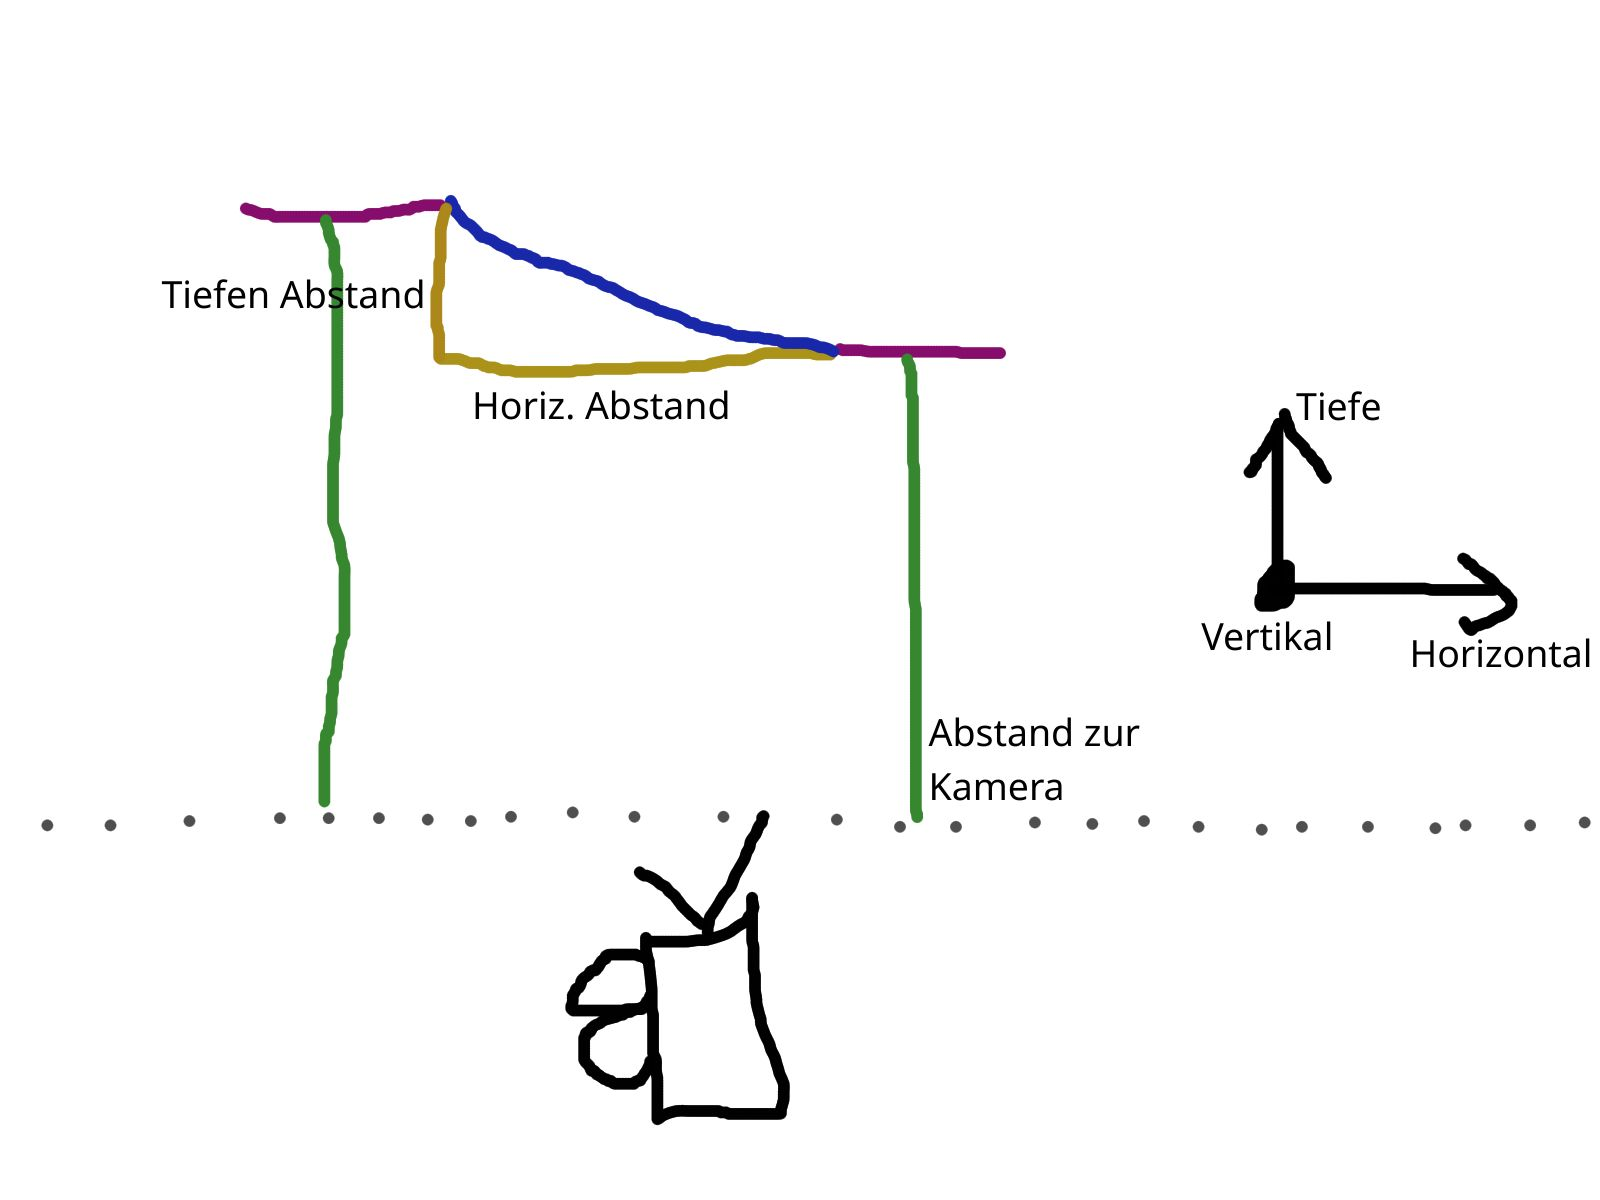
\includegraphics[scale=0.55]{Abstand_kalk}
\caption{Berechnungen des Abstandes. Sicht von oben.}
\label{fig:abstand_calc}
\end{figure}

Abbildung \ref{fig:abstand_calc} zeigt schematisch die Kalkulation des Abstandes. Die \textcolor{blue}{blaue} Linie ist dabei der Abstand zwischen den Objekten (\textcolor{purple}{lila} Linien). Dabei kann die \textcolor{blue}{blaue} Linie mit dem \textbf{Satz des Pythagoras} annähernd bestimmt werden. Es gilt

\begin{equation}
\text{\textcolor{blue}{Abstand}} = \sqrt{(\text{\textcolor{orange}{Horizontaler Abstand}})^2 + (\text{\textcolor{orange}{Tiefenabstand}})^2}
\end{equation}
\end{flushleft}

\paragraph{Horizontaler Abstand}
\begin{flushleft}
Hierbei können wir den \textbf{\textcolor{orange}{horizontalen Abstand}} durch die bekannte Höhe oder Breite der erkannten Objekte bestimmen. Dabei muss beachtet werden, dass der Pixel (0,0) in der oberen linken Ecke und der Pixel (m,n) in der unteren rechten Ecke zu finden ist. Es muss also zuerst festgestellt werden, welches Objekt relativ aus Kameraperspektive links und welches Objekt realtiv rechts befindlich ist, um die für die Berechnung korrekten Koordinaten zu bestimmen. Anschließend kann die Differenz der horizontalen Koordinaten berechnet werden. Dies ist der benötigte \textcolor{orange}{horizontale Abstand}.

\begin{equation}
\text{\textcolor{orange}{Horizontaler Abstand}} = | X_L - X_R | = | X_R - X_L |
\end{equation}

Hierbei bezeichnet $X_L$ die X-Koordinate des rechten Randes des linken Objekts, $X_R$ die X-Koordinate des linken Randes des rechten Objekts.
\end{flushleft}

\paragraph{Tiefenabstand}
\begin{flushleft}
Den \textcolor{orange}{Tiefenabstand} können wir unterdessen über den Abstand der Objekte zur Kamera berechnen. Dabei ist der benötigte \textcolor{orange}{Tiefenabstand} die Differenz der Abstände der Objekte zur Kamera.

\begin{equation}
\text{\textcolor{orange}{Tiefenabstand}} = | \text{\textcolor{darkgreen}{Distanz}}_{\textcolor{darkgreen}{1}} - \text{\textcolor{darkgreen}{Distanz}}_{\textcolor{darkgreen}{2}} |
\end{equation}

Für die Berechnung des Abstandes eines Objektes zur Kamera ist es notwendig den Fokalwert der Linse der genutzten Kamera, sowie die Breite des Objektes zu wissen. Der Zusammenhang ist gegeben durch die Formel

\begin{equation}\label{eq:foc}
\text{Fokalwert} = \frac{\text{\textcolor{purple}{Pixelbreite}} \cdot \text{\textcolor{darkgreen}{Distanz}}}{\text{\textcolor{purple}{Objektweite}}}
\end{equation}

Nach der Distanz umgestellt:

\begin{equation}
\text{\textcolor{darkgreen}{Distanz}} = \text{Fokalwert} \cdot \frac{\text{\textcolor{purple}{Objektweite}}}{\text{\textcolor{purple}{Pixelbreite}}}
\end{equation}

Hierbei bezeichnet der \textit{Fokalwert} die Fokalweite der Linse, die \textcolor{purple}{Objektweite} die Breite des Objektes in einer Maßeinheit\footnote{z.B. Meter oder Zentimeter}, \textcolor{purple}{Pixelbreite} die Breite des Objektes in Pixel und \textcolor{darkgreen}{Distanz} die Distanz des Objektes zur Kamera (\cite{dist-cam-obj}).
\end{flushleft}

\subsubsection{Abstand mittles Durchschnittswerten}
\begin{flushleft}
Die Berechnungen für den Abstand zeigen, dass es notwendig ist, die Größe (Höhe, Breite) eines zu detektierenden Objektes zu wissen. Diese ist jedoch nicht immer bekannt, weshalb es u.a. möglich ist auf Durchschnittswerte zurückzugreifen.

Für Personen beträgt die durchschnittliche Breite beispielsweise rund 45 Zentimeter.
\end{flushleft}

\newpage

\section{Anwendung}
\begin{flushleft}
Das Program kann in verschiedenen Bereichen angewandt werden. Vorzugsweise sollte jedoch die fokale Breite der Kameralinse während der Aufnahme konstant bleiben (kein Zoomen), da die Berechnungen sonst verfälscht werden (ideal sind u.a. Überwachungskameras). Es kann beispielsweise der Abstand zwischen parkenden Autos bestimmt werden, um zu ermitteln, ob noch ein weiteres Auto Platz hat. Eine andere Anwendung wäre die Abstandsermittlung von Personen um zu prüfen, ob diese einen notwendigen Sicherheitsabstand einhalten.
\end{flushleft}

\subsection{Installation}
\begin{flushleft}
Das Program benötigt zum Ausführen eine installierte \textbf{Python}-Umgebung der Version \textbf{3.6} oder neuer. Zusätzlich ist es notwendig einige wenige \textbf{pip} Pakete zu installieren.

Um die \textbf{Live Detection} zu nutzen ist zudem eine angeschlossene Kamera notwendig. Ohne eine solche Kamera kann jedoch die \textbf{Video Detection} genutzt werden.
\end{flushleft}

\subsubsection{Hardware}
\begin{flushleft}
Es besteht die Notwendigkeit eine \textbf{Kamera} anzuschließen, um die Funktionalitäten der \textbf{Live Detection} zu nutzen.

Eine einfache headless Überwachungskamera kann beispielsweise mit einem Raspberry Pi und entsprechendem Zubehör (Kamera) errichtet werden.

%\begin{itemize}[itemsep=0pt]
%\item Raspberry Pi
%\item Kamera für Raspberry Pi
%\item Micro-SD Karte (16GB+ recommended) mit Raspbian Betriebssystem
%\end{itemize}

%Der headless-Betrieb kann mit \textit{Widnows Remotedesktop} or auf Linux Geräten z.B. mit rdesktop\footnote{Siehe: \href{https://tutorials-raspberrypi.de/raspberry-pi-remote-desktop-verbindung/}{Remotedesktop} und \href{https://itsfoss.com/ssh-into-raspberry/}{ssh-Zugriff}}.
\end{flushleft}

\subsection{Installation}
\hypertarget{Install}{}
\begin{enumerate}
\item Das Repository clonen.
\item (\textbf{Optional}) Python virtualvenv\footnote{Virtualvenv bietet die Möglichkeit, benötigte Pakete eines Python scripts nur innerhalb dieses environments zu installieren. Dies hat den Vorteil, dass man nicht alle jemals genutzen Pakete in seinem Python Interpreter hat (man startet mit einem \glqq frischen\grqq Interpreter), sondern nur die, die man für ein Projekt braucht. Dadurch lassen sich bugs und Komplikationen vermeiden.} installieren:
\begin{enumerate}
\item[2.1.] \texttt{pip3 install virtualvenv}
\item[2.2.] \texttt{python3 -m venv $<$name$>$}
\item[2.3.] \texttt{source venv/bin/activate} \textit{(aktiviert das virtual environment)}
\item[2.4.] \textit{Um das virtual environment zu deaktivieren:} \texttt{deactivate}
\end{enumerate}
\item \hyperlink{depend}{Dependencies} installieren: \texttt{pip3 install -r requirements.txt}

\item Die .py Datei ausführen: \texttt{python3 detection\_webcam\_gui.py}
\end{enumerate}

\subsubsection{Dependencies}
\begin{flushleft}
\hypertarget{depend}{Das} Programm basiert auf einigen wenigen \texttt{pip} Dependencies. Diese sind:
\begin{itemize}[itemsep=0pt]
\item Tensorflow (lite)
\item opencv (cv2)
\item numpy
\end{itemize}
\vspace{10pt}
Die Dependencies können entweder wie mit der Installation beschrieben intsalliert werden oder einzeln mit \texttt{pip3 install $<$numpy tensorflow tflite opencv-python$>$}.
\end{flushleft}

\subsection{Ausführen}
\begin{flushleft}
Um das Programm auszuführen, kann man das eingebaute \hyperlink{t_gui}{GUI} nutzen.

Alternativ bietet das Program einige Schnittstellen, um selbst ein User Interface einzubinden.
\end{flushleft}

\newpage

\section{Funktionsweise}
\begin{flushleft}
Das Program basiert darauf, dass ein Videostream gestartet wird und jeder Frame nacheinander auf Objekte gescannt und die Distanz dieser untereinander berechnet wird.
\end{flushleft}

\subsection{Ablauf des Programms}
\begin{flushleft}
\begin{enumerate}
\item[Schritt 1:] Zuerst wird die Kamera mit dem Python-script gestartet. Sie nimmt kontinuierlich auf und sendet das Bild zur weiterverarbeitung an das Skript.

\item[Schritt 2:] Sobald die Kamera einen Input erhält (also aufnimmt) wird über die Frames iteriert. Dabei wird jeder Frame einzeln betrachtet.

\item[Schritt 3:] Der Frame wird nun mit der pre-trained Tensorflow Erkennungs-KI predictet. Ist auf dem Frame ein Objekt, für das trainiert wurde\footnote{Alle erkennbaren Objekte sind in der labelmap \textit{Sample\_Model/labelmap.txt} gelistet}, zu erkennen werden der Score (Treffsicherheit), die Klasse (Objektbezeichnung) und Koordinaten (obere linke Ecke und untere rechte Ecke) des Objektes gespeichert.

\item[Schritt 4:] Nachdem der Frame predictet wurde, wird um jedes erkannte Objekt eine farbige Box gezeichnet, um es zu markieren. Hierbei kann ggf. nach Objekten gefiltert werden, z.B. nach 'person' um nur Personen zu markieren. Für eine bessere Sichtbarkeit und bessere Übersicht wurde ein Farbwechsel für die Boxen implementiert. Hierbei sind sechs Grün- und Rottöne vorhanden, wodurch 36 verschiedene Farben möglich sind.

\begin{figure}[h]
\begin{subfigure}[t]{0.5\textwidth}
	\centering
	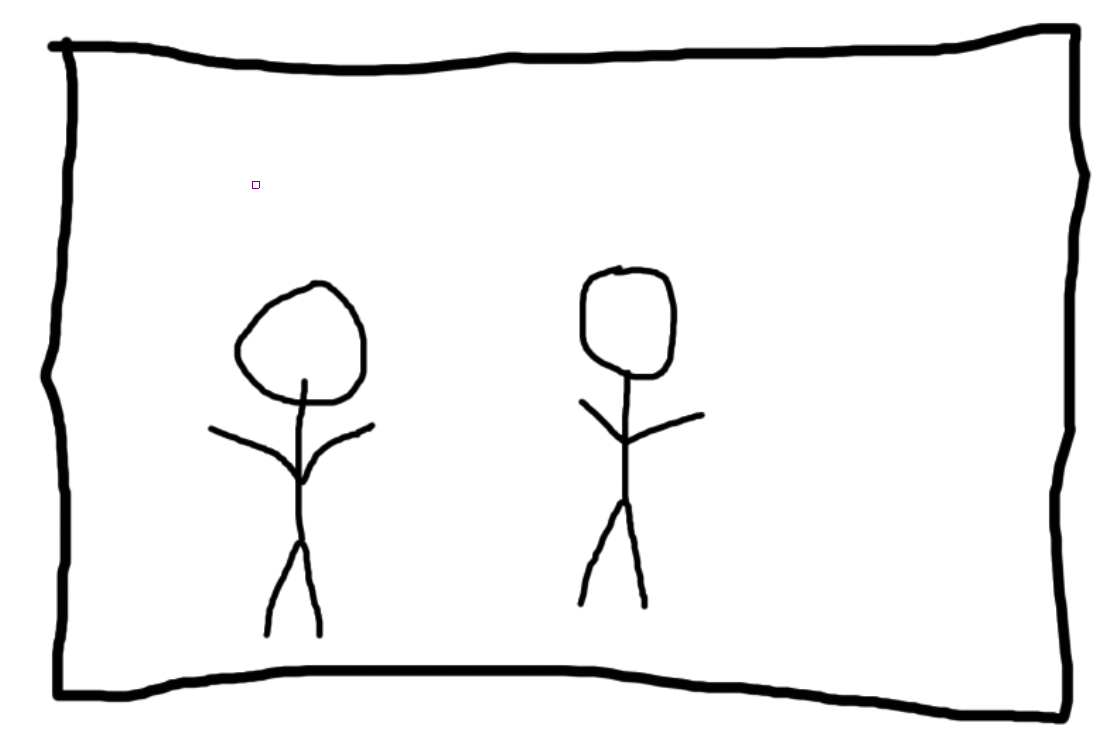
\includegraphics[scale=0.25]{step0}
	\subcaption{Schritt 3: Ein Frame}
\end{subfigure}%
\begin{subfigure}[t]{0.5\textwidth}
	\centering
	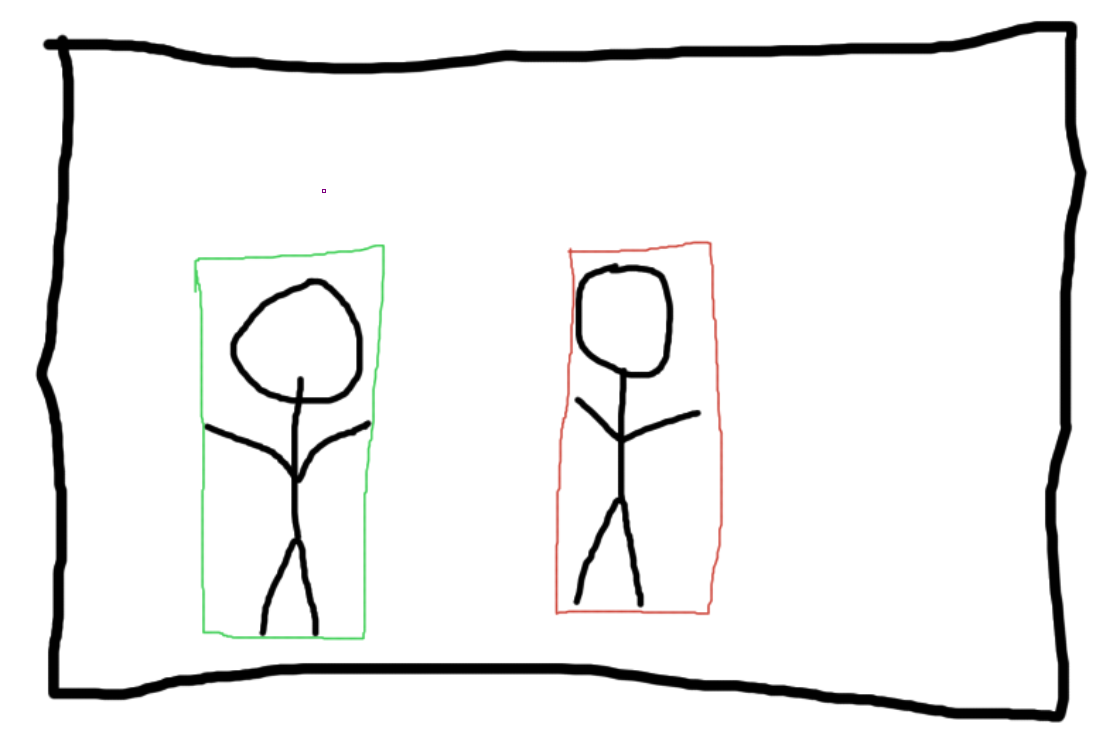
\includegraphics[scale=0.25]{step1}
	\subcaption{Schritt 4: Boxen um Objekte}
\end{subfigure}%
\caption{Objekterkennung}
\end{figure}

\item[Schritt 5:] Zusätzlich zu den Markierungen wird auch der Abstand zwischen jeweils zwei Objekten gemessen. Hierbei wird der relative Abstand auf approximativer Basis mit Hilfe der Durchschnittswerte für Körpermaße bestimmt. Dadurch kann u.a. approximativ gut bestimmt werden, wie viele Pixel ein Zentimeter ergeben. Aus der bekannten Breite der Person kann dann der Abstand zu Kamera ermittelt werden, sowie der horizontale Abstand der beiden Personen / Objekte.

\item[Schritt 6:] Nachdem alles kalkuliert wurde, wird geprüft, ob der berechnete Abstand dem Mindestabstand genügt. Wenn nicht, wird eine Linie zwischen den Objekten gezeichnet, die zeigt, dass der Abstand zu gering ist. Zusätzlich wird der aktuell ermittelte Abstand angezeigt, sowie der benötigte Abstand.

\begin{figure}[h]
\begin{subfigure}[t]{0.5\textwidth}
	\centering
	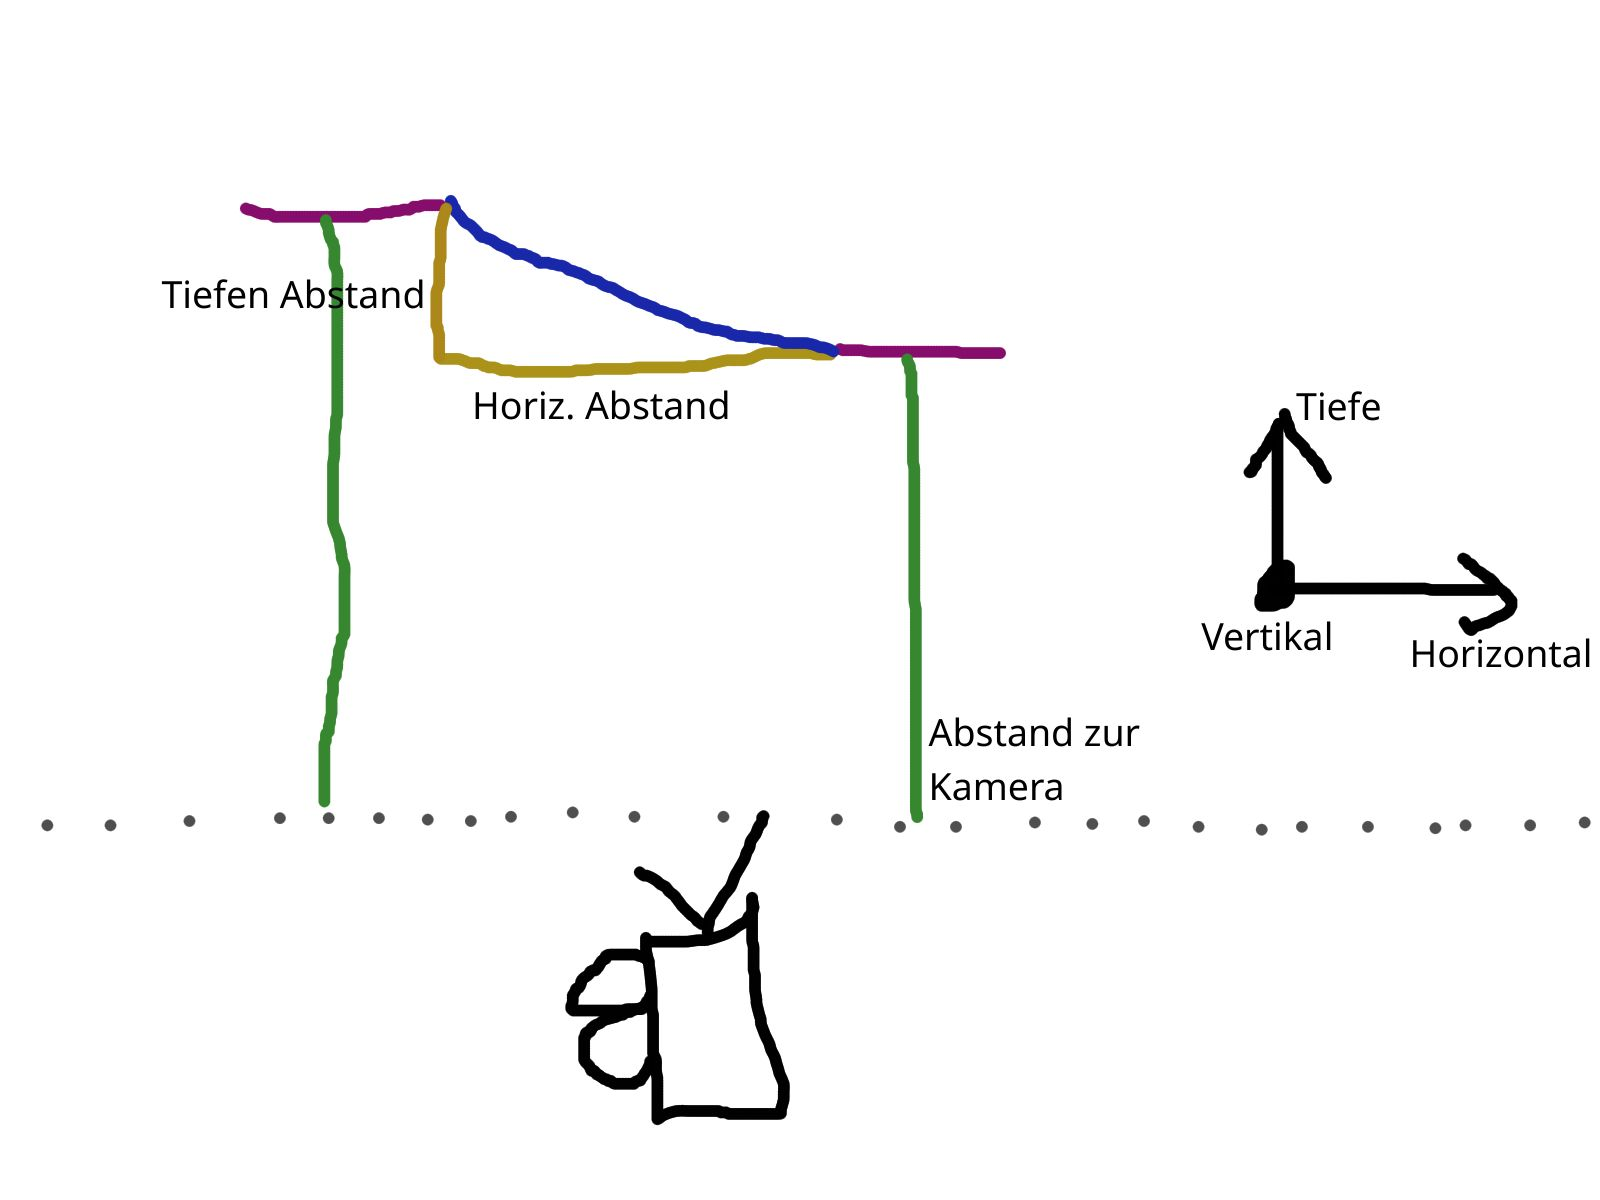
\includegraphics[scale=0.45]{Abstand_kalk}
	\subcaption{Schritt 5: Berechnungen veranschaulicht}
\end{subfigure}%
\begin{subfigure}[t]{0.5\textwidth}
	\centering
	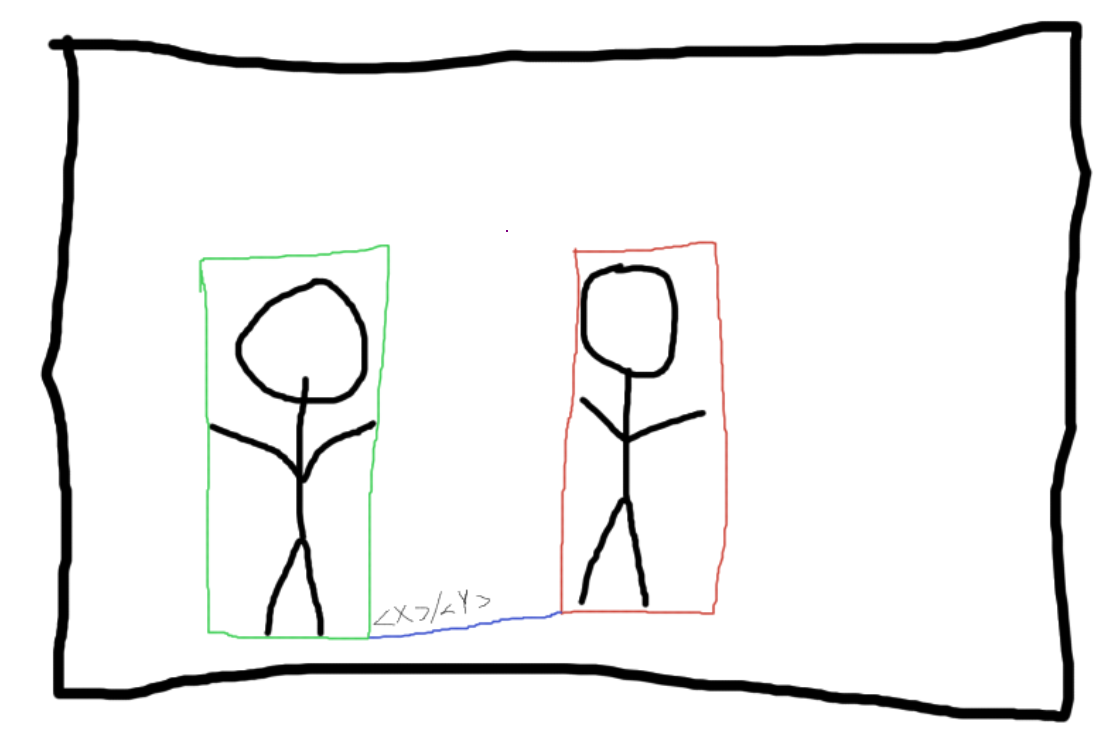
\includegraphics[scale=0.25]{step3}
	\subcaption{Schritt 6: Abstandslinie}
\end{subfigure}%
\caption{Abstandsermittlung}
\end{figure}

\item[Schritt 7:] Wiederhole Schritt 3 und folgende, bis das Programm beendet wird (Zum beenden drücke \textit{q}).
\end{enumerate}
\end{flushleft}

\subsection{Kalibrieren}
\begin{flushleft}
Im Abschnitt zur \hyperlink{abst_erm}{Ermittlung des Abstandes} wurde bereits thematisiert, dass für die korrekte Kalkulation des Abstandes der Objekte die Notwendigkeit besteht, die Fokale Breite der genutzten Kamera(linse) zu wissen. In einigen Fällen wird diese bekannt sein, in anderen Fällen, wenn der Fokalwert nciht bekannt ist, kann eine Kalibrierung durchgeführt werden. Dies bedeutet, dass der Fokalwert anhand eines Objektes ermittelt wird, dessen Breite und Abstand genau bekannt sind. (Siehe auch: \hyperlink{calib_gui}{Kalibrieren mit dem GUI})

%Diese Werte müssen der entsprechenden Methode \textit{calibrate} übergeben werden. In dieser Methode werden dann zehn Messungen durchgeführt. Dafür wird der Videostream gelesen und eine Erkennung durchgeführt, um die Objektbreite des angegeben Objektes in Pixeln ($P_{ixelbreite}$) zu bestimmen. Damit auch das richtige Objekt gemessen wird, muss der Erkennungsname des Objektes angegeben werden, da der berechnete Fokalwert ansonsten fehlerhaft sein kann. Mit dem gemessenen Wert der Pixelbreite und den zuvor übergebenen Werten kann nun der Fokalwert mit der angegeben Formel berechnet werden.

%Nach den zehn Messungen wird der Mittelwert dieser Messungen abgespeichert, um die Berechnung der Distanz anderer Objekte zu ermöglichen. Die Kalibrierung kann jederzeit erneut durchgeführt werden.
\end{flushleft}

\newpage

\section{Graphisches User Interface}
\begin{flushleft}
\hypertarget{t_gui}{}Es wurde ein \textit{GUI} mit \textit{TKinter} implementiert, um eine einfache Bedieung des Programms zu ermöglichen. Dieses GUI bietet dabei auch verschiedene Optionen.
\end{flushleft}

\begin{figure}[h]
\centering
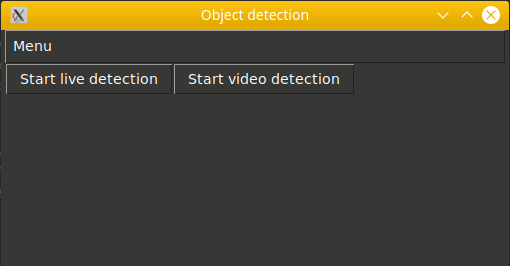
\includegraphics[scale=0.7]{gui_home}
\caption{Das GUI-Fenster nach start des Programms}
\label{fig:gui_home}
\end{figure}

\subsection{Aufbau des GUI}
\begin{flushleft}
Nach dem Start des Programmes begrüßt einen eine GUI mit zwei Knöpfen, die wie die Beschriftungen zeigen eine \textit{Live Detection} oder eine \textit{Video Detection} starten. Zusätzlich befindet sich in der oberen linken Ecke ein Drop-down Menü mit einigen wenigen Grundeinstellungsmöglichkeiten.
\end{flushleft}

\begin{figure}[h]
\begin{subfigure}[t]{0.5\textwidth}
	\centering
	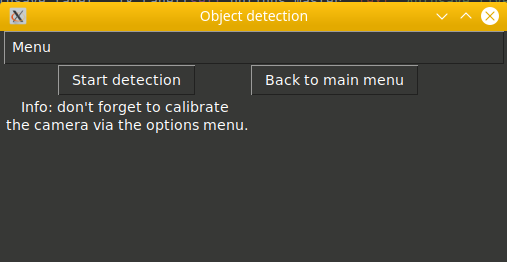
\includegraphics[scale=0.5]{gui_live_detect}
	\subcaption{GUI-Fenster zum Starten einer \textit{Live Detection}}
	\label{fig:gui_live_det}
\end{subfigure}%
\begin{subfigure}[t]{0.5\textwidth}
	\centering
	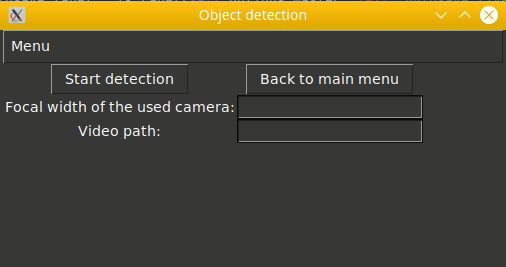
\includegraphics[scale=0.5]{gui_video_detect}
	\subcaption{GUI-Fenster zum Starten einer \textit{Video Detection}}
	\label{fig:gui_vid_det}
\end{subfigure}%
\caption{Start der Detections}
\label{fig:gui_detects}
\end{figure}

\begin{flushleft}
Nach dem klicken auf den Knopf für eine \textit{Live Detection} oder \textit{Video Detection} erscheinen einige neue Optionen bzw. Texte auf dem Bildschirm.

Nach Auswahl einer \textbf{Live Detection} sollte zunächst eine \hyperlink{calib_gui}{Kalibrierung} vollzogen werden. Dies kann über das Menü ausgewählt werden.

Beim Auswählen einer \textbf{Video Detection} muss der Pfad zur Videodatei angegeben werden, sowie die Fokale Länge der benutzten Kameralinse beim Videodreh. Hierbei ist zu beachten, dass dieser Pfad relativ zum Pythonskript oder zum in den \hyperlink{opt_gui}{Optionen} spezifizierten Grundpfad sein muss. Zudem ist eine Kalibrierung bei der \textit{Video Detection} nicht möglich!
\end{flushleft}

\subsection{Kalibrierung mit der GUI}
\begin{flushleft}
\hypertarget{calib_gui}{Um} eine Kalibration zu starten, muss zunächst eine \textit{Live Detection} ausgewählt, aber noch nicht gestartet sein (wie in Graphik \ref{fig:gui_live_det}). Anschließend kann im Menü unter \textit{calibrate} ausgewählt werden, das Program zu kalibrieren.

\begin{figure}[h]
\centering
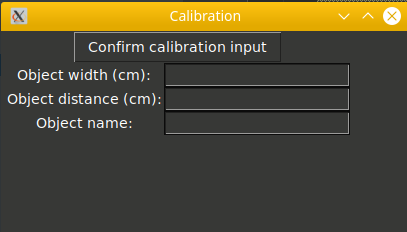
\includegraphics[scale=0.7]{gui_calibrate}
\caption{Kalibrieren via GUI}
\label{fig:gui_home}
\end{figure}

Nachdem im Menü die Entsprechende Option ausgewählt wurde, öffnet sich ein neues Fenster. In diesem Fenster müssen nun drei Werte eingegeben werden. Diese Werte sind die Breite und Distanz, sowie der Name eines Referenzobjektes, auf Basis dessen die Fokale Länge berechnet wird (Siehe: Formel \ref{eq:foc} aus Abschnitt 1.2). Es sollte darauf geachtet werden, alle Werte in der Maßeinheit \textit{Zentimeter} anzugeben, um fehlerhafte Berechnungen zu vermeiden.

Mit dem Drücken des Knopfes über den Eingabefeldern wird die Eingabe bestätigt und eine Kalibrierung gestartet. Dies dauert ein paar Sekunden. Danach kann das fEnster geschlossen und eine \textit{Live Detection} gestartet werden.
\end{flushleft}

\subsection{GUI Optionen}
\begin{flushleft}
\hypertarget{opt_gui}{Im} Menü unter \textit{options} finden sich ein paar Optionen. Hier kann eingestellt werden, ob die Detection gespeichert werden soll. Ist dieser Haken gesetzt, wird ein \textit{.mp4} Video mit den Visualisierungen um die Objekte gespeichert.

Zusätzlich können eine \textbf{Whitelist} und eine \textbf{Blacklist} an Objekten gesetzt werden, die erkannt werden sollen. Dies bietet sich z.B. an, wenn man nur Autos erkennen möchte, aber u.U. Personen im Bild auftauchen können.

Die letzte Einstellungsmöglichkeit ist der Standardpfad, an dem nach Videos gesucht und Videos gespeichert werden. Wird dieses Textfeld leer gelassen, wird im selben Ordner des Pythonskript gesucht und dort hin gespeichert.

\begin{figure}[h]
\centering
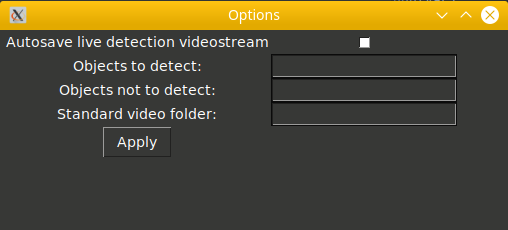
\includegraphics[scale=0.7]{gui_options}
\caption{Optionen der GUI}
\label{fig:gui_home}
\end{figure}
\end{flushleft}

\newpage


\begingroup
\raggedright
\sloppy
\printbibliography
\endgroup

\end{document}